\documentclass{article}
\usepackage{tikz}
\usetikzlibrary{arrows, shapes, positioning}
\tikzstyle{nodeobserved} = [circle, minimum size = 10mm, thick, draw =black!80]
\usetikzlibrary{external}
\tikzexternalize

\begin{document}

\begin{figure}
    \centering

    \tikzsetnextfilename{dag-bmi}
    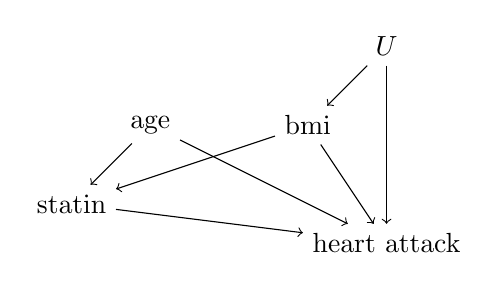
\begin{tikzpicture}
      % Nodes
      \node (bmi) at (1, 1) {bmi};
      \node (age) at (-1, 1) {age};
      \node (u) at (2, 2) {$U$};
      \node (t) at (-2, 0) {statin};
      \node (y) at (2, -0.5) {heart attack};

      % Edges
      \draw[->] (u) -- (bmi);
      \draw[->] (u) -- (y);
      \draw[->] (age) -- (t);
      \draw[->] (bmi) -- (t);
      \draw[->] (age) -- (y);
      \draw[->] (bmi) -- (y);
      \draw[->] (t) -- (y);

    \end{tikzpicture}

\end{figure}

\end{document}
